% !TEX program = xelatex
\documentclass{article}
\usepackage{geometry}
\geometry{left = 2.5cm, right = 2.5cm, top = 3cm, bottom = 3cm}
\usepackage[linesnumbered,ruled,longend]{algorithm2e}
\usepackage{amsmath}
\usepackage[makeroom]{cancel}
\usepackage{amsfonts,amssymb}
\usepackage{tcolorbox}
\usepackage{blkarray}
\usepackage{booktabs}
\usepackage{colortbl}
\usepackage{dsfont}
\usepackage{enumerate}
\usepackage{extarrows}
\usepackage{epsf}
\usepackage{fontspec}
\usepackage{forest}
\usepackage[colorlinks=true,linkcolor=purple]{hyperref}
\usepackage{listings}
\usepackage{mathrsfs}
\usepackage{microtype}
\usepackage{multirow}
\usepackage{setspace}
\usepackage{tikz}
\usepackage{xcolor}
\tcbuselibrary{skins}
\newcommand\Ccancel[2][black]{\renewcommand\CancelColor{\color{#1}}\cancel{#2}}
\newcommand{\Sangle}[1]{\langle {#1} \rangle}
%\usepackage{indentfirst}
%\usepackage[usenames,dvipsnames]{xcolor}
\newfontfamily\Inputmono{Consolas}
\renewcommand\thesection{Note\ \arabic{section}}%\arabic{section}}
\renewcommand\thesubsection{\roman{subsection}).}
\numberwithin{equation}{section}
\renewcommand{\theequation}{\arabic{section}.\arabic{equation}}
% \renewcommand\thesubsubsection{\roman{subsection}).\alph{subsubsection}.}
\newcommand{\qedhere}{$\hfill\ensuremath{\square}$}
\newcommand{\f}{\frac}
\newcommand{\<}{\langle}
\newcommand{\p}{\partial}
\newcommand\supp{{\rm supp\ }}
\defaultfontfeatures{Mapping=tex-text,Scale=MatchLowercase}
\newcommand\mycommfont[1]{\ttfamily\textcolor{blue}{#1}}
\SetCommentSty{mycommfont}
%\setmainfont{Citadel Script}
%\setmainfont{Chalkboard}
\setmainfont{CMU Bright}
%\setmainfont{Apple Chancery}
\setmonofont{Optima}
\setsansfont{Optima}
%\renewcommand{\familydefault}{\sfdefault}
%\renewcommand{\footnotesize}{\sfdefault}
\setlength{\parskip}{0.25em}
\setlength{\parindent}{0em}

%%%%%%%%%%%Configurations for code%%%%%%%%%%%%%%%%%%%%%%%
\SetKwInOut{Input}{Input}
\SetKwInOut{Output}{Output}
\SetKwProg{Fn}{Function}{\string:}{end}
\SetKwFunction{mstnew}{MST\_New}
\SetKwFunction{tw}{TreeWeight}
\SetKwFunction{dps}{DFS}
\SetKwFunction{con}{Is\_Connected}
\SetKwFunction{hor}{Three\_Fastest\_Horses}


%%%%%%%%%%%Here is the configurations for Code%%%%%%%%%%%

\definecolor{mygreen}{rgb}{0,0.6,0}
\definecolor{mygray}{rgb}{0.7,0.7,0.7}
\definecolor{mymauve}{rgb}{0.58,0,0.82}
\definecolor{mywhite}{rgb}{1,1,1}
\definecolor{myblack}{rgb}{0,0,0}
\definecolor{myblue}{RGB}{27,154,154}
\lstset{
backgroundcolor=\color{white},
basicstyle = \footnotesize\Inputmono,
breakatwhitespace = false,
breaklines = true,
captionpos = b,
commentstyle = \color{mygray}\bfseries,
extendedchars = false,
frame =shadowbox,
framerule=0.5pt,
frameround=tttt,
keepspaces=true,
keywordstyle=\color{myblue}\bfseries, % keyword style
language = Verilog,                     % the language of code
otherkeywords={string},
numbers=left,
numbersep=5pt,
numberstyle=\tiny\color{mymauve},
rulecolor=\color{black},
showspaces=false,
showstringspaces=false,
showtabs=false,
stepnumber=0,
stringstyle=\color{mymauve},        % string literal style
tabsize=2,
title=\lstname
}

%%%%%%%%%%%%%%%%%%%%%%%%%%%%%%%%%%%%%%%%%%%%

\begin{document}
%\setmainfont{Savoye LET}
%\setmainfont{Cormorant Upright}
\setmainfont{Cormorant Upright}
\renewcommand\arraystretch{1.5}


\thispagestyle{empty}

\begin{center}
\begin{large}
\begin{figure}[!htbp]
\centering
\includegraphics[width=0.7\textwidth]{Logo2}
\end{figure}
\hrule
\vspace*{0.25cm}
\sc{ \Large  UM--SJTU Joint Institute \vspace*{0.3em}} \\
\Large  VV557 Methods of Applied Math II\\
\end{large}
\hrulefill

\vspace*{2cm}
\begin{Large}
\sc{{Lecture Notes Hints}} \\
\end{Large}
\vspace*{2cm}
\begin{Large}

\end{Large}
\vspace*{0.5cm}
\begin{large}
\sc{collected by \textbf{Tianze, Wang}}
\end{large}
\end{center}
\newpage

\begin{center}
\vspace*{6em}
Page Left blank because I want to.
\end{center}

\newpage
\setmainfont{Optima}
\setmonofont{Optima}
\setsansfont{Optima}
%\tableofcontents
%\newpage
\setcounter{page}{1}
\normalsize
\section{Boundary Value Problems of Higher order $p$}
\begin{tcolorbox}[colback=blue!10!white]
An example problem:
\begin{align}
	L = D^2(b_2 D^2)+ D(b_1 D)+b_0
\end{align}
where $b_2,b_1,b_0$ are functions of $x$.
\end{tcolorbox}
We first calculate conjunction and $L^*$. Apply integral chain rule,
\begin{align}
	\int v L u &= \int v[(b_2 u'')''+(b_1 u')'+ b_0]\notag\\
	\int v(b_2u'')'' &= v(b_2 u'')'-\int v'(b_2u'')'\notag \\
	&=v(b_2 u'')'-v'(b_2u'') +\int v''b_2u'' \notag\\
	&= v(b_2 u'')'-v'(b_2u'')+u'v''b_2-u(v''b)' +\int(v''b_2)''y \label{conjunu''} \\
	\int v(b_1 u')' &= v(b_1u')-\int v'(b_1u')\notag \\
	&=v(b_1u')-ub_1v'+ \int u(b_1v')'' \label{conjunu'}
\end{align}
We synthesis \eqref{conjunu''} and \eqref{conjunu'}, which yields to 
\begin{align}
	L^* = L
\end{align}
and 
\begin{align}
	J(u,v) = v(b_2 u'')'-v'(b_2u'')+u'v''b_2-u(v''b)'+v(b_1u')-ub_1v'|_a^b
\end{align}
\begin{tcolorbox}[colback=red!5!white, boxrule = 0.1pt]
Two cases to be considered as self adjoint.
\begin{itemize}
	\item $u(a),u''(a),u(b),u''(b)=0$ 
	\item $u(a),u'(a),u(b),u'(b)=0$
\end{itemize}
However, if three conditions for $a$ and one condition for $b$, not self-adjoint. \textit{This could be easily verified as plug in the conditions and see what need to happen to make conjunction to be 0 for $v$.}
\end{tcolorbox}
\section{Solvability Conditions}
Solve \begin{align} L u &=\delta(x-\xi)-v^{(1)}(\xi) v^{(1)}(x)-\cdots-v^{(k)}(\xi) v^{(k)}(x) \\ &=: f(x) \end{align}
instead of originally $L u  = \delta(x- \xi)$
\section{Partial Boundary Value Problems General Notes}
\subsection{Basic Quantities}
\begin{tcolorbox}[colback=blue!10!white]
\begin{equation}
	L u :=-\nabla\cdot (p(x) \nabla u)+q(x) u
\end{equation}
\end{tcolorbox}
\subsection{Derivation of Green's Formula}
\begin{tcolorbox}[colback=green!10!white]
Green's Formula is given as
\begin{equation}
	\int_{\Omega}(v L u-u L v) d x = \int_{\partial \Omega} p\left(u \frac{\partial v}{\partial n}-v \frac{\partial u}{\partial n}\right) d \sigma
\end{equation}
\end{tcolorbox}
The steps are: According to divergence delta rule
\begin{equation}
	\nabla \cdot(f \vec{v})=f(\nabla \cdot \vec{v})+\vec{v} \cdot(\nabla f)
\end{equation}
Rearrange the items, it will lead to
\begin{equation}
	f(\nabla \cdot \vec{v})=\nabla \cdot(f \vec{v})-\vec{v} \cdot(\nabla f)
\end{equation}
where as $f = p$ and $\vec v = p \nabla u$
\section{PP 330}
To calculate a surface integral in $\mathbb{R}^n$ of $S\subset \mathbb{R}^n$ is a hypersurface.
\subsection{Step 1: Find parametrization $\gamma$}
\begin{align*}
	\gamma :[a_1,b_1]\times ... \times [a_{n+1},b_{n+1}] \rightarrow S \subset \mathbb{R}^n \\
	\gamma: (s_1,...,s_{n+1}) \mapsto \begin{pmatrix}
	\gamma_1(s_1,...s_{n+1})\\
	\gamma_2(s_1,...s_{n+1})\\
	\gamma_3(s_1,...s_{n+1})\\
	\vdots \\
	\gamma_{n+1}(s_1,...s_{n+1})\\
	\end{pmatrix} 
\end{align*}

\begin{tcolorbox}[colback=blue!20!white]
A simple example is given as
\begin{align*}
(\phi, \theta) = \begin{pmatrix}
	\cos \pi \sin \theta\\
	\sin \pi \sin \theta\\
	\cos \theta
\end{pmatrix}
\end{align*}
\end{tcolorbox}
\subsection{Step 2: Find a normal vector $\vec{n}\perp S$}
\subsection{}
\begin{align*}
	\int_S f ds = \int \int \int ...\int f(\gamma(s_1,...,s_{n+1})) \det(\frac{\partial \gamma}{\partial s_1},...,\vec{a})
\end{align*}

\section{PP 366}
\begin{align*}
	\int_{\varphi} f ds = \int_a^b f \circ \gamma(t)\cdot  |\gamma'(t)|dt
\end{align*}
where $\varphi$ indicates curve/line integral on $\mathbb{R}^n$. by
\[
	\gamma (t) = \begin{pmatrix}
		t \\ 0
	\end{pmatrix}
\]
$t \in R$, $\gamma'(t) = \begin{pmatrix} 1\\0 \end{pmatrix}$, $|\gamma'(t) | = 1$.
So
\begin{align*}
	&\int_{\partial \mathbb{H}} h(\cdot ) \frac{\partial g(x;\cdot )}{\partial n} ds \\
	&= \int_{-\infty}^\infty h(\gamma(t))\cdot \frac{-\partial g(x;\cdot )}{\partial \xi_2}|_{\gamma(t)} dt \\
	&= - \int _{- \infty }^{\infty}h(\xi_2)\cdot \frac{-\partial g(x;\xi_1,\xi_2 )}{\partial \xi_1}|_{\xi_2 = 0} dt \\
\end{align*}

\section{Method of Images}
\begin{tcolorbox}[colback=green!10!white]
This part is to raise an intuitive understanding of \textbf{Method of Images} chapter.
\end{tcolorbox}
Electrostatics by Maxwell
\[
	- \Delta \underbrace{V}_{\text{potential}} = 4 \pi \underbrace{\rho}_{\text{charge density}}
\]
For a unit point charge located at $\xi$, it has charge density $\delta(x- \xi)$. The potential for a point charge is
\begin{align*}
	V(x;\xi) = \frac{1}{4 \pi \varepsilon_0}\cdot  \frac{1}{|x-\xi|}
\end{align*}

This solves $-\Delta V = 4 \pi \delta(x-\xi)$

\begin{tcolorbox}[colback = blue!10!white]
E.g. a charge of 1 Coulomb at $\xi$ and 2 Coulomb at $\xi^*$,
\[
	- \Delta V = 4 \pi (\delta(x- \xi)+ 2 \delta(x- \xi^*))
\]
which is also taken as 
\[
	V = V_1 + V_2
\]
where according to the superposition principle
\begin{align}
	- \Delta V_1 = - 4 \pi \delta(x- \xi) \label{eqn1} \\
	- \Delta V_2 = - 4 \pi \delta(x- \xi^*) \label{eqn2} 
\end{align}
If $V_1$ solves equation \eqref{eqn1}, $V_2$ also solves equation \eqref{eqn2}. 
\[
	V_2(x; \xi^*) = 2 V_1(x;\xi^*)
\]
The effect of having a \textbf{ground plate} at x plane is equal to have a $\xi^*$ charge.
\end{tcolorbox}
\section{Neumann Problem}
\begin{align}
	\frac{\partial g}{\partial n} = 0 \quad g = \text{physical potential} \label{eqn4}
\end{align}
which means g satisfy $\Delta g = \delta$ and boundary condition.
\begin{equation}	
	\Sangle{\nabla g, \vec{n}} = 0 \label{eqn3}
\end{equation}
This equation means the force perpendicular to the boundary vanishes. This equation \eqref{eqn3} means at boundary the force is 0. Please note that for Neumann problems, the potential at boundary points is arbitrary as long as \eqref{eqn4} is satisfied.

\section{PP 374}
\setcounter{equation}{0}
\begin{center}
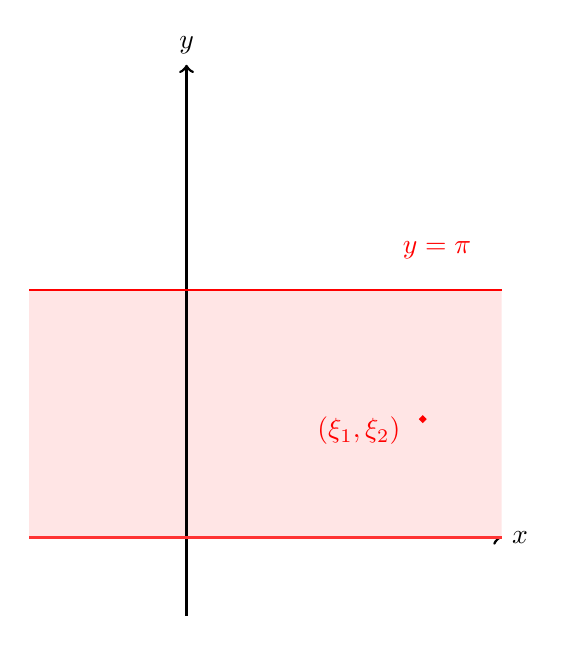
\begin{tikzpicture}[domain=-2:4,line width=1pt]
    \draw[->] (-2,0) -- (4,0) node[right] {$x$};
    \path[fill = red!10!white] (-2,0) -- (4,0) -- (4,3.14) -- (-2,3.14) --(-2,0);
    \draw[->] (0,-1) -- (0,6) node[above] {$y$};
	\draw[domain = -2:4,color=red] plot (\x,{3.14})
       node[above=0.5cm, left = 0.25cm] {$y = \pi$};
    \draw[fill, color = red] (3,1.5) circle [radius = 0.025]
    	node[below = 0.15cm,left = 0.15cm] {$(\xi_1,\xi_2)$};
    \draw[draw = red!80!white] (-2,0) --(4,0) ;
\end{tikzpicture}
\end{center}
\begin{tcolorbox}
Consider the reflection of $\xi$ according to two boundaries.
\end{tcolorbox}
We have 
\begin{equation}
	\Delta g = \delta(x - \xi), g|_{\partial \Omega} = 0
\end{equation}
So 
\begin{equation}
	E(x,\xi) = \frac{1}{2 \pi} \ln |x- \xi|
\end{equation}
and the sequence of images are 
\begin{equation*}
	\xi_n^{\pm} = (\xi_1, \pm \xi_2 \pm 2 n \pi)
\end{equation*}

Then we have 
\begin{align}
	g(x;\xi) &= \sum_{n \in \mathbb{Z}} E(x, \xi_n^+) - \sum_{n \in \mathbb{Z}} E(x, \xi_n^-) \notag \\
	&= \frac{1}{2 \pi} \sum_{n \in \mathbb{Z}} \ln |x- \xi_n^+| -\frac{1}{2 \pi} \sum_{n \in \mathbb{Z}} \ln |x- \xi_n^-| 
\end{align}
\begin{tcolorbox}[colback=green!20!white]
Two comments:
\begin{enumerate}
	\item We ignore convergence issue
	\item Introduce complex numbers:
	\begin{align}
	\left|\begin{pmatrix}
			x_1 \\ x_2
		\end{pmatrix}\right| = |x_1+ ix_2| = \sqrt{x_1^2+x_2^2}
	\end{align}
\end{enumerate}
\end{tcolorbox}
Then we could write 
\begin{align*}
	|x- \xi_n^+| = \left| \begin{pmatrix}
		x_1 \\ x_2
	\end{pmatrix} - \begin{pmatrix}
		\xi_1 \\ \xi_2 + 2n \pi
	\end{pmatrix}\right| 
	& = |(x_1 -\xi_1) + (x_2- \xi_2 + 2 n \pi)i| \\
	& = |x - \xi + 2 n \pi i| \quad x = x_1 + x_2 i
\end{align*}
Similarly,
\[
	|x - \xi_n^-| = |x - \bar{\xi} + 2n \pi i ||
\]
So we have 
\begin{align}
	\sum_{n \in \mathbb{Z}} \ln |x - \xi_n^+| = \sum_{n \in \mathbb{Z}} \ln |x - \xi+ 2n \pi i| = \ln \left( \prod _{n \in \mathbb{Z} } |x- \xi + 2n \pi i|\right)
\end{align}
Now 
\begin{align}
	g(x , \xi) & = \frac{1}{ 2 \pi} \ln \left( \prod _{n \in \mathbb{Z} }  \frac{|x- \xi + 2n \pi i|}{ |x- \bar{ \xi}+ 2n \pi i|}\right) \notag\\
	&= \frac{1}{2 \pi} \ln \left| \left(\prod _{n \in \mathbb{Z} } \frac{\frac{x -\xi}{2 i n \pi}-1 }{\frac{x - \bar{\xi}}{2 n \pi i}-1}\right) \cdot \frac{x - \xi}{x - \bar\xi} \right|
\end{align}
According to Weierstraß factorization theorem,
\begin{align}
	&\sinh(z) = \frac{e^z - e^{-z}}{2} \notag \\
	&\sinh(ix) = -i \sin(x) \notag \\
	&\sinh(z) = 2\cdot \prod_{n \in Z \backslash 0} (z - i n \pi) = 2 \prod_{ n \in \mathbb{Z}\backslash 0}(1- \frac{z}{i n \pi}) \label{eqnhp}
\end{align}
Here \ref{eqnhp} is to evaluate hyperbolic function. 
And we have
\begin{align}
	g(x, \xi) &= \frac{1}{2 \pi} \ln \left| \frac{\sinh((x- \xi)/2	)}{\sinh((x- \bar\xi)/2)} \right| \notag\\
	&= \frac{1}{4 \pi} \ln\left|\frac{\sinh^2((x- \xi)/2)}{\sinh^2((x- \bar\xi)/2)}\right| \label{shit}
\end{align}
Also, we have an equation
\begin{align}
	\sinh^2 (a+bi) = \cosh^2(a) - \cos^2(b) \label{sincosh}
\end{align}
Plug \eqref{sincosh} into \eqref{shit}
it yields to 
\begin{align}
	g(x,\xi) = \frac{1}{4 \pi} \ln \left( \frac{\cosh^2((x_1 - \xi_1)/2) + \cos^2 ((x_2 - \xi_2)/2)}{\cosh^2((x_1 - \xi_1)/2) + \cos^2 ((x_2 + \xi_2)/2)} \right)
\end{align}
Then in this case
\begin{align}
	u(x) &= \int_{\delta \Omega} \frac{\partial g(x,\cdot )}{\partial n}|_{\partial \Omega} \cdot f \label{px2}\\
	\frac{\partial g}{\partial n} &= \langle \nabla g, \hat n\rangle \notag \\
	&= \langle \begin{pmatrix} \frac{\partial g}{\partial \xi_1} \\ \frac{\partial g}{\partial \xi_2} \end{pmatrix} , \pm \begin{pmatrix}0 \\ 1\end{pmatrix}  \rangle \notag \\
	&= \pm \frac{\partial g}{\partial \xi_2} 
\end{align}
Plug in $\xi_2 = \pi$ into \eqref{px2}
\begin{align}
	\frac{\partial g}{\partial \xi_2} |_{\xi_2 = \pi} = \frac{1}{2 \pi} \frac{sin(x_2)}{cos(x_1 - \xi_1)+ cos(x_2)}
\end{align}
So the final answer
\[
	u(x) = \frac{\sin(x_2)}{2 \pi} \int_{-\infty} ^{+\infty} \left(\frac{f_1(\xi_1)}{\cosh(x_1 - \xi_1)+ \cos(x_2)}+\frac{f_2(\xi_1)}{\cosh(x_1 - \xi_1)- \cos(x_2)}\right) d \xi_1
\]
\begin{tcolorbox}[colback=blue!10!white]
\begin{center}
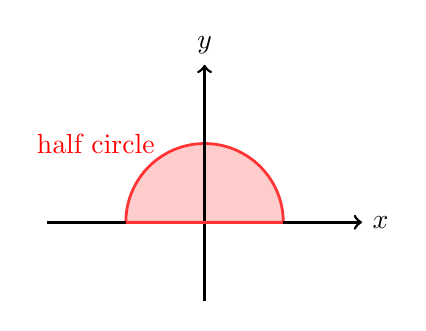
\begin{tikzpicture}[domain=-2:2,line width=1pt]
    \filldraw[fill=red!20!white, draw = red!80!white] (0,0) -- (1,0) arc (0:180:1) -- cycle
       node[above=1cm, left = 0.5cm, color = red] {half circle};
    \draw[->] (-2,0) -- (2,0) node[right] {$x$};
    \draw[->] (0,-1) -- (0,2) node[above] {$y$};
    \draw[draw = red!80!white] (-1,0) --(1,0) ;
	% \draw[domain = -1:1,color=red] plot (\x,{sqrt(1-\x*\x)})
    % \draw[fill, color = red] (3,1.5) circle [radius = 0.025]
    % 	node[below = 0.15cm,left = 0.15cm] {$(\xi_1,\xi_2)$};
\end{tikzpicture}
\end{center}
Partial Eigenfunction Expansion	(Draw a semi circle with boundary to be red here)
$- \Delta g = \delta, \quad g|_{\partial \Omega} = 0$
\end{tcolorbox}
\begin{align}
	\Delta_{(r,\theta)} = \frac{\partial^2}{\partial r^2} + \frac{1}{r} \cdot \frac{\partial}{\partial r} + \frac{1}{r^2} \frac{\partial^2}{\partial \theta^2}
\end{align}
\begin{enumerate}[1)]
\item First find partial eigenfunctions
$- \Delta u = 0$, $u = u(r, \theta) = R(r) \cdot \Theta(\theta)$
\begin{align}
	&\frac{\partial^2}{\partial r^2}  R \Theta+ \frac{1}{r} \cdot \frac{\partial}{\partial r} R \Theta+ \frac{1}{r^2} \frac{\partial^2}{\partial \theta^2}R \Theta = 0 \notag \\
	\Leftrightarrow&R''\Theta+ \frac{1}{r}R'\Theta+ \frac{1}{r^2}R \Theta'' = 0\notag\\
	\Leftrightarrow & \frac{r^2}{R}R''+ \frac{r}{R}R' = - \frac{\Theta''}{\Theta} = \lambda \in \mathbb{R}
\end{align}
Then we transform into an eigenvalue problem
\begin{align}
	&\Theta''+ \lambda \Theta = 0  &0 < \Theta < r\\
	& r^2 R'' + r R' - \lambda R = 0 &0 < r < 1, R(1) = 0
\end{align}
\item Choose and find a set of eigenfunctions
\begin{align}
	\Theta_m(\theta) = \underbrace{\sqrt{\frac{2}{\pi}}}_{\text{Normalize coordinate}} \cdot \sin(m \theta),\qquad m \in \mathbb{N}^*
\end{align}
\item Expand the unknown green function in terms of eigenfunction
\begin{align}
	g(r, \theta; \rho, \varphi)& = \sum_{n=1}^{+\infty } g_m(r, \rho , \varphi)\cdot \Theta_m(\theta) \\
	g_m(r, \rho , \varphi) &= \sqrt{\frac{2}{\pi}} \int_{0}^\pi g(r, \theta; \rho, \varphi) \sin(m \theta) d \theta 
\end{align}
\item Determine the ODE Green's function problem
\begin{align}
	- \Delta_{(r, \theta)}g(r, \theta; \rho, \varphi) = \frac{\delta(r- \rho) \delta(\theta - \varphi)}{r} \label{star}
\end{align}
Multiply \eqref{star} with $\frac{2}{\pi} \sin(m \theta)$, then integrate
\begin{align}
 	&- \int \frac{2}{\pi} \sin(m \theta) \left(\Delta_{(r, \theta)} g\right) = \frac{2 }{\pi r} \sin(m \varphi) \delta(r - \rho) \notag\\
 	\Leftrightarrow & - \left(\frac{\partial^2}{\partial v^2}+ \frac{1}{r} \frac{\partial}{\partial r}\right) g_m(r, \rho, \varphi) - \frac{1}{r^2} \int_0^ \pi \frac{2}{\pi} \sin(m \theta) \cdot  \frac{\partial^2 g}{\partial \theta^2} d \theta = \frac{2 }{\pi r} \sin(m \varphi) \delta(r - \rho) \notag\\
 	\Leftrightarrow & - \frac{\partial^2}{\partial r^2} g_m + \frac{1}{r} \frac{\partial}{\partial r} g_m + \frac{m^2}{r^2} g_m = \frac{2 }{\pi r} \sin(m \varphi) \delta(r - \rho) 
\end{align} 
Consider $g_m = g_m(r)$, then we can write this as 
\begin{align}
	-r^2 g_m'' + r g_m + m ^2 g_m = \frac{2 }{\pi} r \sin(m \varphi)\cdot \delta(r - \rho)
\end{align}
Note that here
\begin{align*}
	r\cdot \delta(r- \rho) = \rho\cdot \delta( r - \rho)
\end{align*}
which is due to
\begin{align}
	r T_{\delta(r- \rho)} \varphi = T_{\delta(r- \rho)} (r \cdot \varphi(r)) = \rho\cdot \varphi(\rho)
\end{align}
Now we choose $g_m$ to satisfy
\begin{align*}
	g_m|{r = 0} = g_m|{r=1} = 0
\end{align*}
\begin{tcolorbox}
Here for $r=0$, we cannot choose $g_m$ arbitrarily. At the origin, $\theta$ is not properly defined, 
\end{tcolorbox}
\item Solve it !
\begin{align}
	&-r^2g_m''-rg_m'+m^2g_m = 0 \notag
	\\&\qquad\Rightarrow g_m(r) = r^\lambda \Rightarrow \lambda = \pm m 
\end{align}
Then find $g_m$.
\begin{equation}g_m(r, \rho, \varphi) = \left\{
\begin{aligned}
	&\frac{1}{m}\frac{r^m(\rho^{-m} - \rho^m)}{\pi} \sin(m \varphi) \qquad r < \rho\\
	&\frac{1}{m}\frac{\rho^m(r^{-m} - r^m)}{\pi} \sin(m \varphi) \qquad r > \rho
	\end{aligned}
	\right.
\end{equation}
\item Put it together
\begin{equation}
	g(r,\theta; \rho, \varphi) = \sum_{m=1}^\infty g_M(r, \rho, \varphi) \sin(m \theta)
\end{equation}
\end{enumerate}
\section{HW5 EX3}
The Fourier expansion can be 
\begin{align}
	f(x)  = c_0 \langle f, 1 \rangle &+ \sum_{n=1}^\infty c_n \langle f, \cos(nx) \rangle \cos(nx) \\&+
	\sum_{n=1}^{\infty}d_n \langle f, \sin(nx) \rangle \sin(nx)
\end{align}
\section{HW5 EX5}
iv.
\begin{align}
	u(x) = \int_0^1 g_M(x,\xi) f(\xi) d \xi + c_0 + c_1 x
\end{align}
\section{HW6 EX2}
\begin{align}
	u_{tt} - u_{xx} = F(x,t) \qquad u(x,0) = f(x) \quad u_t(x,0) = h(x)
\end{align}
The greens formula work for bounded regions. 
\begin{center}
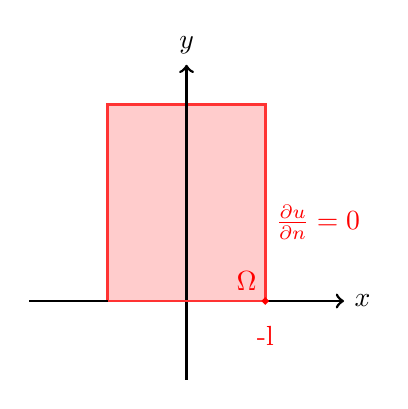
\begin{tikzpicture}[domain=-2:2,line width=1pt]
    \filldraw[fill=red!20!white, draw = red!80!white] (0,0) -- (1,0) -- (1,2.5) -- (-1, 2.5) --(-1,0) --cycle
       node[above = 0.25cm, right = 0.5cm, color = red] {$\Omega$};
    \draw[->] (-2,0) -- (2,0) node[right] {$x$};
    \draw[->] (0,-1) -- (0,3) node[above] {$y$};
    \draw[draw = red!80!white] (-1,0) --(1,0) ;
    \draw[fill, color = red] (1,0) circle [radius = 0.025] node [above = -0.7cm] {-l};
    \draw[fill, color = red] (1,1) node[right] {$\frac{\partial u}{\partial n} = 0$};
	% \draw[domain = -1:1,color=red] plot (\x,{sqrt(1-\x*\x)})
    % \draw[fill, color = red] (3,1.5) circle [radius = 0.025]
    % 	node[below = 0.15cm,left = 0.15cm] {$(\xi_1,\xi_2)$};
\end{tikzpicture}
\end{center}
\begin{align*}
	&B_1^* u = u(x,T)\\
	&B_2^* u = u_t(x,T)
\end{align*}
Now we have 
\begin{align}
	\langle u, Lv \rangle - \langle v, Lu \rangle &= \iint u(x,t)[v_{tt} - v_{xx}]-v[u_{tt}-u_{xx}] dxdt \notag \\
	&= \int _{-L}^L \int _0^T (uv_{tt}-vu_{tt}) dtdx - \int_0^T\int_{-L}^L(uv_{xx}-vu_{xx})dxdt \notag \\
	&= \int_{-L}^L [uv_t|_0^T - \Ccancel[red]{\int _0^T u_tv_tdt} - vu_t|_0^T+ \Ccancel[red]{\int_0^T u_tv_tdt}]-... \notag \\
	&= \int_{-L}^L (u v_t- vu_t)|_0^T dx - \int_0^T (u_xv_x-vu_x)|_{-L}^L dt\notag \\
	&= \int_{-L}^L \int_0^T \frac{d}{dt}(u v_t- v u_t) dt dx - \int_0^T \int_{-L}^L \frac{d}{dx}(uv_x-vu_x) dx dt\notag \\
	&= \iint_{\Omega} div_{(x,t)} \underbrace{\begin{pmatrix}v u_x - uv_x\\ uv_t-vu_t\end{pmatrix}}_{J(u,v)} d (x,t) 
\end{align}
\begin{tcolorbox}
Recall that green's function 
\begin{align}
	\langle u,Lv \rangle- \langle v,Lu \rangle = \int Jd \vec\sigma  
	\Sangle{a}
\end{align}
Recall the Causal F.S.:
\begin{equation}
	E(x,t;\xi,\tau) = \frac{1}{2}H(t - \tau- |x- \xi|)
\end{equation}
\end{tcolorbox}

Adjoint boundary conditions
\begin{align}
	M= \{ u \in C^2 (\Omega) \cap C(\bar\Omega) u(x,0) = 0, u_t(x,0) =0, u_x(-L,t) = u_x(L,t) = 0\}
\end{align}
Solution formula:
\begin{itemize}
	\item u satisfies
	\begin{equation}
		u_{xx}-u_{tt} = 0, \quad u(x,0) = f(x), \quad u_t(x,0) =h(x), u_x(\pm L,t) = 0
	\end{equation}
	\item v satisfies
	\begin{equation}
		v_{xx}-v_{tt} = \delta, \quad v(x,T) =0, \quad v_t(x,T) = 0, \quad v_x(\pm L,t) = 0
	\end{equation}
	Also we have 
	$v = g^*$
\end{itemize}
So here we have 
\begin{align}
	\Sangle{u,Lv} - \Sangle{v,Lu} &= u(\xi) - \int_\Omega g^* F \notag \\
	&= \int_{-L}^L u(x,0)g_t^*(x,0) - u_t(x,0) g^*(x,0) dx 
\end{align}
Then 
\begin{align}
	u(\xi, \tau) = \int_ \Omega g^*(x,t; \xi, \tau ) F(x,t) d(x,t) + \cdots  \label{xtfixed}
\end{align}
Fix $\xi$ and $\tau$, For $L$ large enough, at the boundary, the conditions for $\partial u/ \partial n = 0$ automatically satisfies.
\begin{align}
	E( \pm L, t; \xi, \tau) &= \frac{1}{2} H(t- \tau - |\pm L - \xi| ) = 0 \qquad \text{ if $L$ large} \label{t-0}\\
	E(x,0;\xi,\tau) &= \frac{1}{2} H(T - \tau- |x- \xi|) = 0 \label{t+0}
\end{align}
Equation \eqref{t+0} is always 0 because $\tau>0$. From \eqref{t-0} and \eqref{t+0}, we can conclude \[
	E \in M
\]
We take 
\begin{equation}
	E^*(x,t;\xi,\tau) = E(\xi,\tau;x,t)
\end{equation}
as $g^*$. So that \eqref{xtfixed} can be then expressed as
\begin{align}
	u(\xi, \tau) &= \int_ \Omega g^*(x,t; \xi, \tau ) F(x,t) d(x,t) + \cdots \notag\\
	&= \iint_\Omega \frac{1}{2} H(\tau - t - |x- \xi|) F(x,t) d(x,t) + \cdots \label{beforextt} \\
	&= \frac{1}{2} \int_0^\tau \int_{\xi-(\tau-t)}^{\xi+(\tau-t)}F(x,t) dxdt \label{afterxtt}
\end{align}
From \eqref{beforextt} to \eqref{afterxtt}, it is due to the equation evaluates to 1 only if
\[
	|x- \xi| <\tau - t
\]
\section{Adjoint and direct boundary conditions for PDE}
Direct Boundary conditions
\begin{align}
	M = \{u \in C^2 (V): Bu = \tilde{B}_1u=0\}
\end{align}
Here
\begin{align}
	&Bu = \gamma(x,t) \quad (x,t) \in \partial \Omega\times (0,\infty)\\
	&\tilde{B}_1u = u(x,0) = f(x)
\end{align}
Adjoint Boundary condition
\begin{align}
	M^* = {v\in C^2(V),B^*v = \tilde{B}^*_1 v = 0}
\end{align}
where 
\begin{align}
	&B^*v = Bv\\
	&\tilde{B}_1^*v = v(x,T)
\end{align}
\section*{}
Modified greens' function
Non-separapble ODE
\textbf{Method of Images, Eigenvalue}
\section{How to solve these fucking problems in Chpter 4}
\subsection{Solvability}
\begin{enumerate}
\item Find adjoint problem: For adjoint problem, it has the same \textbf{trivial or non-trivial} solution as the original problem.
\item check $\int fv = 0$.
\item If $\int fv = 0$, it means that the function is solvable. Otherwise, it's not solvable.
\item Then we need to use modified green function.
\begin{align}
\begin{aligned} \operatorname{Lg}_{M}(x, \xi) &=\delta(x-\xi)-\sum_{i=1}^{k} v^{(i)}(\xi) v^{(i)}(x) \\ B_{1} g_{M} &=0 \\ \vdots & \\ B_{p} g_{M} &=0 \end{aligned}
\end{align}
Note here $v$ is orthonormal solution.
\item The modified adjoint green function is 
\begin{align}
\begin{aligned} L^{*} g_{M}^{*}(x, \xi) &=\delta(x-\xi)-\sum_{i=1}^{k} u^{(i)}(\xi) u^{(i)}(x) \\ B_{1}^{*} g_{M}^{*} &=0 \\ \vdots & \\ B_{p}^{*} g_{M}^{*} &=0 \end{aligned}
\end{align}
\item Then the final solution is given as
\begin{align}
u(x)=\int_{a}^{b} g_{M}(x, \xi) f(\xi) d \xi+\sum_{i=1}^{k} c_{i} u^{(i)}(x)
\end{align}
\end{enumerate}
\end{document}















